\documentclass[doubleside, titlepage]{article}
\usepackage{xcolor,listings}
\usepackage[utf8]{inputenc}
\usepackage[english]{babel}
\usepackage{textcomp}
\usepackage{graphicx}
\usepackage[papersize={210mm,297mm},top=2cm, bottom=2.25cm, left=1.8cm , right=1.8cm]{geometry}
\lstset{upquote=true}
\usepackage{amsmath}
\usepackage{tikz}
\usepackage{epigraph}
\usepackage{hyperref}
\hypersetup{
    linktoc=all
}
\usepackage{titlesec}
\usepackage{fancyhdr}
\pagestyle{fancy}
\usepackage{lastpage}

\renewcommand\headrulewidth{0.66pt}
\fancyhead[L]{\leftmark}
\fancyhead[R]{Spring 2016}

\renewcommand\footrulewidth{0.66pt}
\fancyfoot[L]{ ~\\ Group 3}
\fancyfoot[C]{ ~\\CS323 - Deliverable 1 \\ \textbf{Page \thepage/\pageref{LastPage}}}
\fancyfoot[R]{ ~\\ 
\includegraphics[scale=0.35]{epfl_logo}}

\fancypagestyle{firstpage}{%
    \fancyhf{}%
    \renewcommand\footrulewidth{0.66pt}
    \fancyfoot[L]{ ~\\ Group 3}
    \fancyfoot[C]{ ~\\CS323 - Deliverable 1 \\ \textbf{Page \thepage/\pageref{LastPage}}}
    \fancyfoot[R]{ ~\\ 
\includegraphics[scale=0.35]{epfl_logo}}
    \renewcommand{\headrulewidth}{0mm}%
} 

\renewcommand\epigraphflush{center}
\renewcommand\epigraphsize{\normalsize}
\setlength\epigraphwidth{0.5\textwidth}
\setlength\epigraphrule{0.5pt}

\renewcommand{\textflush}{flushright} \renewcommand{\sourceflush}{flushright}

\let\originalepigraph\epigraph 
\renewcommand\epigraph[2]{\originalepigraph{#1}{\textsc{#2}}}

\definecolor{titlepagecolor}{cmyk}{0,.9,0.7,0}

\DeclareFixedFont{\titlefont}{T1}{ppl}{b}{}{0.5in}

\makeatletter                       
\def\printauthor{%                  
    {\large \@author}}              
\makeatother
\author{%
	~\\	~\\
    Jeremy Hottinger \\
    259573 \\
    \href{mailto:jeremy.hottinger@epfl.ch}{\texttt{jeremy.hottinger@epfl.ch}}\vspace{20pt} \\
    Aurélien Soccard \\
    235746 \\
    \href{mailto:aurelien.soccard@epfl.ch}{\texttt{aurelien.soccard@epfl.ch}}\vspace{20pt} \\
    Téo Stocco \\
    235744 \\
    \href{mailto:teo.stocco@epfl.ch}{\texttt{teo.stocco@epfl.ch}}\vspace{20pt} \\
    }

% The following code is borrowed from: http://tex.stackexchange.com/a/86310/10898

\newcommand\titlepagedecoration{%
\begin{tikzpicture}[remember picture,overlay,shorten >= -10pt]

\coordinate (aux1) at ([yshift=-15pt]current page.north east);
\coordinate (aux2) at ([yshift=-410pt]current page.north east);
\coordinate (aux3) at ([xshift=-4.5cm]current page.north east);
\coordinate (aux4) at ([yshift=-150pt]current page.north east);

\begin{scope}[titlepagecolor!40,line width=12pt,rounded corners=12pt]
\draw
  (aux1) -- coordinate (a)
  ++(225:5) --
  ++(-45:5.1) coordinate (b);
\draw[shorten <= -10pt]
  (aux3) --
  (a) --
  (aux1);
\draw[opacity=0.6,titlepagecolor,shorten <= -10pt]
  (b) --
  ++(225:2.2) --
  ++(-45:2.2);
\end{scope}
\draw[titlepagecolor,line width=8pt,rounded corners=8pt,shorten <= -10pt]
  (aux4) --
  ++(225:0.8) --
  ++(-45:0.8);
\begin{scope}[titlepagecolor!70,line width=6pt,rounded corners=8pt]
\draw[shorten <= -10pt]
  (aux2) --
  ++(225:3) coordinate[pos=0.45] (c) --
  ++(-45:3.1);
\draw
  (aux2) --
  (c) --
  ++(135:2.5) --
  ++(45:2.5) --
  ++(-45:2.5) coordinate[pos=0.3] (d);   
\draw 
  (d) -- +(45:1);
\end{scope}
\end{tikzpicture}%
}

\begin{document}
\begin{titlepage}
\thispagestyle{firstpage}
\vspace*{3cm}
\titlefont CS-323 : Deliverable 1\par
\vspace*{0.5cm}
\epigraph{This is our first deliverable for the \textit{Bookshelf} project of the introduction to database course (spring 2016 - Pr. Anastasia Ailamaki), which sums up our ER-model and schema. It also contains some justifications.}%
{\textit{March 2016} - \textsc{Team n°3}}
\null\vfill
\vspace*{5cm}
\noindent
\hfill
\begin{minipage}{0.5\linewidth}
    \begin{flushright}
        \printauthor
    \end{flushright}
\end{minipage}
%
\begin{minipage}{0.02\linewidth}
    \rule{1pt}{175pt}
\end{minipage}
\titlepagedecoration
\end{titlepage}

\setcounter{tocdepth}{1}
\vspace{-1cm}
\tableofcontents

~\\
\noindent\rule[0.5ex]{\linewidth}{0.25pt}

\section{Justifications}

We started to take a look at the given data and tried to understand how tables where connected at a first glance by drawing a really simplified diagram. Once this was done, we started to look at more deeply to the data : how are they stored? May they be empty? Are they all relevant? Our major decision was not to drop any table, but only add and remove some fields to entities.
~\\~\\
First, for everything that is related to publications, we quickly figured out how things were working. Therefore, we quickly decided to drop some of the unused id (such as its author or its content). As a primary key, we made the choice to inflate it using constraints. Furthermore, we also decided to separate the price into two fields, one for the amount and one for the currency, this solution being much more efficient while looking for some price range for instance. 
~\\~\\
Another part of the work was to analyse how tables were connected to remove potential redundancy. For instance, an award has a category but also a type, and a category has a type. These two types being always the same, we needed to drop out some content, what we've done by removing the type entry in a award. We also realise that, for instance in the author table, among the 80'000 birth places, only 10\% were unique so we have started thinking about changing this attribute into a placeID and create a places table. There were some advantages (no redundancy, less space consumed) but some drawbacks (2 queries instead of one for each author) that finally made us stay with the given configuration (however, if another would be using a place, we will have done that).
~\\~\\
Furthermore, to write properly the creation of the table, we needed to know exactly what entry may be null, and which ones could not. This was done by inspecting carefully the data and reading correctly the instructions. Then, the dilemma was for notes and web pages tables. Indeed, for note, we only have two entries : the ID and the raw note, whereas for a website, there are an ID, an URL but also some other IDs to relate it to other entities : among these 7 IDs, only one   The type of each entry is explained in the following paragraph. Our final has been not the change the structure of these two tables since there is no WebpageID entry in tables as there is for note, but whether a web page is directly connected to the ID of its corresponding entity. Therefore, it implies to add an entry into these 7 tables, and we decided not to do this for practical reasons. Besides, we also thought about simply adding a simply URL entry into the note table, but this solution was also not satisfactory since before insert we would need to do a map from web page to note (not that hard) but since primary keys are only unique in one table, an author and a publication may have the same ID and this would imply much more work to know which website belongs to who.
~\\~\\
Last but not least, some intensive parsing has also been performed to know exactly how many characters were required for instance for each field, since we have encountered some difficulties with Cyrillic. We quickly realised that we should definitely parse these values before inserting them, it presents the advantages of being less memory consuming (6 characters become 1) and also the process of conversion is only done one time.
\addtocounter{page}{1}

\section{ER model}

This entity-relation model only contains fields which are either directly use for relation or as primary key (underline then). For a more complete view of the table, refers to the next section. Fields are coloured in blue, direct relationships in yellow, relationships through a table in red.
~\\
\textbf{Note :} If you find this diagram too small, a larger version is available online at the following address : 
$$
\text{\href{https://documents.epfl.ch/users/s/so/soccard/private/DBMS}{\texttt{https://documents.epfl.ch/users/s/so/soccard/private/DBMS}}}
$$
\begin{flushright}
(access restricted to the db2016 group as defined in the EPFL AD directory).
\end{flushright}

\newpage

\begin{center}
    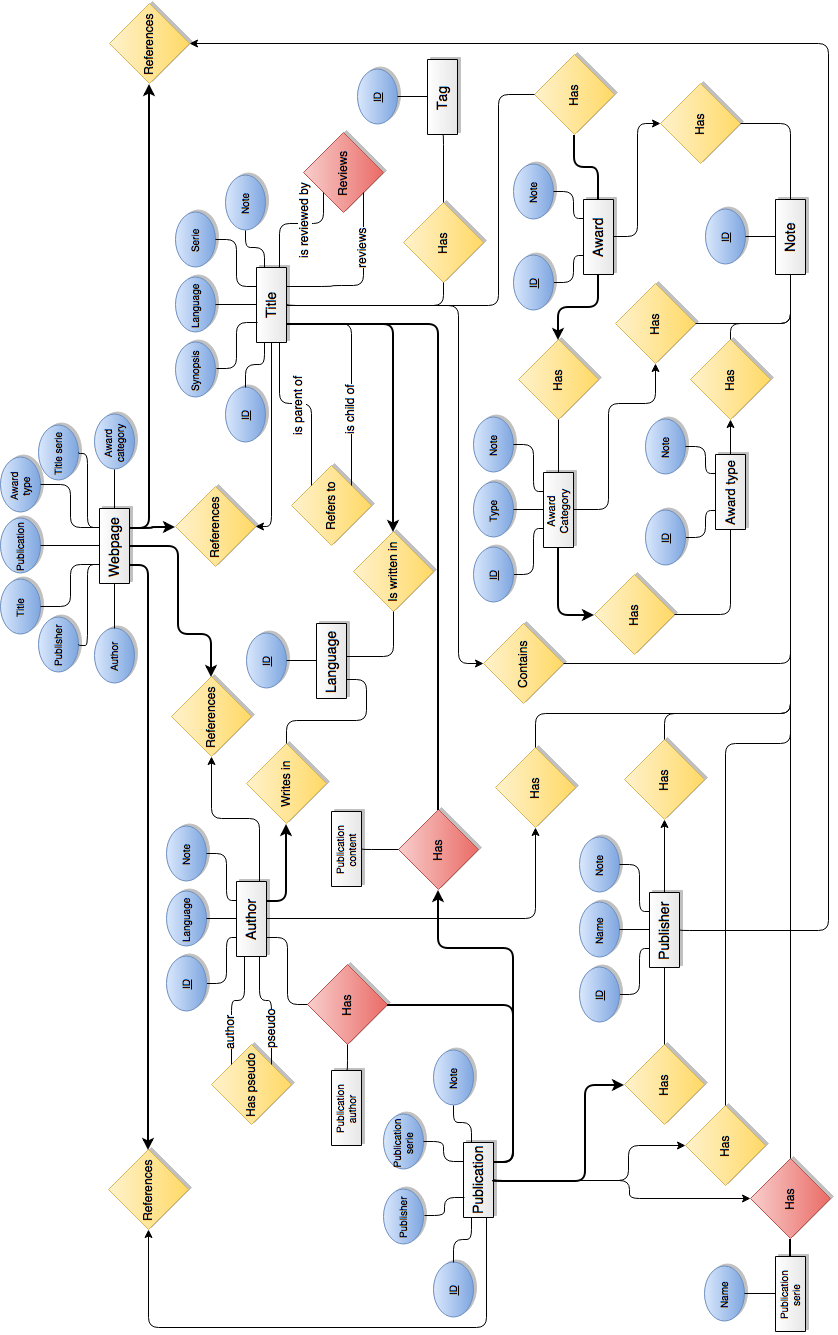
\includegraphics[scale = 0.5]{DBMS_ER}
\end{center}

\section{SQL schema}

\subsection{Entities}

\begin{lstlisting}[language=SQL,showspaces=false,basicstyle=\ttfamily,numberstyle=\tiny,commentstyle=\color{gray}
        ]
CREATE TABLE authors
(
  id          INT PRIMARY KEY NOT NULL,
  name        VARCHAR(256)    NOT NULL,
  legal_name  VARCHAR(256),
  last_name   VARCHAR(256),
  pseudonym   INT, -- fk
  birth_place VARCHAR(256),
  birth_date  DATE,
  death_date  DATE,
  email       VARCHAR(256),
  image       VARCHAR(256),
  language_id INT, -- fk
  note_id     INT -- fk
)
\end{lstlisting}

\begin{lstlisting}[language=SQL,showspaces=false,basicstyle=\ttfamily,numberstyle=\tiny,commentstyle=\color{gray}
        ]
CREATE TABLE publications
(
  id             INT PRIMARY KEY NOT NULL,
  title          VARCHAR(256)    NOT NULL,
  date_pub       DATE            NOT NULL,
  publisher_id   INT             NOT NULL, -- fk
  pages          INT,
  preface        INT,
  packaging_type VARCHAR(256)    NOT NULL,
  type           VARCHAR(256)    NOT NULL,
  isbn           INT UNIQUE,
  cover          VARCHAR(256),
  price          FLOAT,
  currency       VARCHAR(256),
  pub_series_id  INT, -- fk
  pub_series_num INT,
  note_id        INT -- fk
)
\end{lstlisting}

\begin{lstlisting}[language=SQL,showspaces=false,basicstyle=\ttfamily,numberstyle=\tiny,commentstyle=\color{gray}
        ]
CREATE TABLE titles
(
  id           INT PRIMARY KEY NOT NULL,
  title        VARCHAR(256)    NOT NULL,
  translator   VARCHAR(256),
  synopsis     INT, -- fk
  note_id      INT, -- fk
  series_id    INT, -- fk
  series_num   INT,
  story_length VARCHAR(256),
  type         VARCHAR(256),
  parent       INT             NOT NULL DEFAULT 0, -- fk
  language_id  INT, -- fk
  graphic      BOOLEAN         NOT NULL
)
\end{lstlisting}

\newpage

\begin{lstlisting}[language=SQL,showspaces=false,basicstyle=\ttfamily,numberstyle=\tiny,commentstyle=\color{gray}
        ]
CREATE TABLE languages
(
  id     INT PRIMARY KEY NOT NULL,
  name   VARCHAR(256)    NOT NULL,
  code   CHAR(3)         NOT NULL UNIQUE,
  script BOOLEAN
)
\end{lstlisting}

\begin{lstlisting}[language=SQL,showspaces=false,basicstyle=\ttfamily,numberstyle=\tiny,commentstyle=\color{gray}
        ]
CREATE TABLE notes
(
  id   INT PRIMARY KEY NOT NULL,
  note TEXT            NOT NULL
)
\end{lstlisting}

\begin{lstlisting}[language=SQL,showspaces=false,basicstyle=\ttfamily,numberstyle=\tiny,commentstyle=\color{gray}
        ]
CREATE TABLE webpages
(
  id                     INT PRIMARY KEY NOT NULL,
  author_id              INT, -- fk
  publisher_id           INT, -- fk
  title_id               INT, -- fk
  url                    VARCHAR(256)    NOT NULL UNIQUE,
  publications_series_id INT, -- fk
  award_type_id          INT, -- fk
  title_series_id        INT, -- fk
  award_category_id      INT -- fk
)
\end{lstlisting}

\begin{lstlisting}[language=SQL,showspaces=false,basicstyle=\ttfamily,numberstyle=\tiny,commentstyle=\color{gray}
        ]
CREATE TABLE tags
(
  id   INT PRIMARY KEY NOT NULL,
  name VARCHAR(256)    NOT NULL
)
\end{lstlisting}

\begin{lstlisting}[language=SQL,showspaces=false,basicstyle=\ttfamily,numberstyle=\tiny,commentstyle=\color{gray}
        ]
CREATE TABLE titles_series
(
  id      INT PRIMARY KEY NOT NULL,
  title   VARCHAR(256)    NOT NULL,
  parent  INT DEFAULT 0, -- fk
  note_id INT -- fk
)
\end{lstlisting}

\begin{lstlisting}[language=SQL,showspaces=false,basicstyle=\ttfamily,numberstyle=\tiny,commentstyle=\color{gray}
        ]
CREATE TABLE awards
(
  id          INT PRIMARY KEY NOT NULL,
  title       VARCHAR(256)    NOT NULL,
  date        DATE            NOT NULL,
  category_id INT             NOT NULL, -- fk
  note_id     INT -- fk
)
\end{lstlisting}

\begin{lstlisting}[language=SQL,showspaces=false,basicstyle=\ttfamily,numberstyle=\tiny,commentstyle=\color{gray}
        ]
CREATE TABLE awards_categories
(
  id      INT PRIMARY KEY NOT NULL,
  name    VARCHAR(256)    NOT NULL,
  type_id INT             NOT NULL, -- fk
  ordr    INT,
  note_id INT -- fk
)
\end{lstlisting}

\newpage

\begin{lstlisting}[language=SQL,showspaces=false,basicstyle=\ttfamily,numberstyle=\tiny,commentstyle=\color{gray}
        ]
CREATE TABLE awards_types
(
  id          INT PRIMARY KEY NOT NULL,
  code        CHAR(2) UNIQUE,
  name        VARCHAR(256)    NOT NULL,
  note_id     INT, -- fk
  awarded_by  VARCHAR(256)    NOT NULL,
  awarded_for VARCHAR(256)    NOT NULL,
  short_name  VARCHAR(256)    NOT NULL UNIQUE,
  poll        BOOLEAN         NOT NULL,
  non_genre   BOOLEAN         NOT NULL 
)
\end{lstlisting}

\begin{lstlisting}[language=SQL,showspaces=false,basicstyle=\ttfamily,numberstyle=\tiny,commentstyle=\color{gray}
        ]
CREATE TABLE publishers
(
  id      INT PRIMARY KEY NOT NULL,
  name    VARCHAR(512)    NOT NULL,
  note_id INT -- fk
)
\end{lstlisting}

\begin{lstlisting}[language=SQL,showspaces=false,basicstyle=\ttfamily,numberstyle=\tiny,commentstyle=\color{gray}
        ]
CREATE TABLE publications_series
(
  id      INT PRIMARY KEY NOT NULL,
  name    VARCHAR(512)    NOT NULL,
  note_id INT -- fk
)
\end{lstlisting}

\subsection{Relations}

\begin{lstlisting}[language=SQL,showspaces=false,basicstyle=\ttfamily,numberstyle=\tiny,commentstyle=\color{gray}
        ]
CREATE TABLE publications_authors
(
  publication_id INT NOT NULL, -- fk
  author_id      INT NOT NULL, -- fk
  CONSTRAINT pk_publications_authors PRIMARY KEY (publication_id, author_id)
)
\end{lstlisting}

\begin{lstlisting}[language=SQL,showspaces=false,basicstyle=\ttfamily,numberstyle=\tiny,commentstyle=\color{gray}
        ]
CREATE TABLE titles_awards
(
  title_id INT NOT NULL, -- fk
  award_id INT NOT NULL, -- fk
  CONSTRAINT pk_titles_awards PRIMARY KEY (title_id, award_id)
)
\end{lstlisting}

\begin{lstlisting}[language=SQL,showspaces=false,basicstyle=\ttfamily,numberstyle=\tiny,commentstyle=\color{gray}
        ]
CREATE TABLE titles_tags
(
  title_id INT NOT NULL, -- fk
  tag_id   INT NOT NULL, -- fk
  CONSTRAINT pk_titles_tags PRIMARY KEY (title_id, tag_id)
)
\end{lstlisting}

\begin{lstlisting}[language=SQL,showspaces=false,basicstyle=\ttfamily,numberstyle=\tiny,commentstyle=\color{gray}
        ]
CREATE TABLE reviews
(
  title_id  INT NOT NULL, -- fk
  review_id INT NOT NULL, -- fk
  CONSTRAINT pk_reviews PRIMARY KEY (title_id, review_id)
)
\end{lstlisting}

\newpage

\begin{lstlisting}[language=SQL,showspaces=false,basicstyle=\ttfamily,numberstyle=\tiny,commentstyle=\color{gray}
        ]
CREATE TABLE publications_contents
(
  title_id       INT NOT NULL, -- fk
  publication_id INT NOT NULL, -- fk
  CONSTRAINT pk_publications_contents PRIMARY KEY (title_id, publication_id)
)
\end{lstlisting}


\subsection{Foreign keys}

\subsubsection{Authors}
\begin{tabular}{ ll }
\begin{minipage}{3in}
\begin{lstlisting}[language=SQL,showspaces=false,basicstyle=\ttfamily,numberstyle=\tiny,commentstyle=\color{gray}
        ]
ALTER TABLE authors
ADD FOREIGN KEY (language_id)
REFERENCES languages (id)
ON DELETE SET NULL;
\end{lstlisting}
\end{minipage}
&
\begin{minipage}{3in}
\begin{lstlisting}[language=SQL,showspaces=false,basicstyle=\ttfamily,numberstyle=\tiny,commentstyle=\color{gray}
        ]
ALTER TABLE authors
ADD FOREIGN KEY (pseudonym)
REFERENCES authors (id)
ON DELETE CASCADE;
\end{lstlisting}
\end{minipage}
\\
\begin{minipage}{3in}
\begin{lstlisting}[language=SQL,showspaces=false,basicstyle=\ttfamily,numberstyle=\tiny,commentstyle=\color{gray}
        ]
ALTER TABLE authors
ADD FOREIGN KEY (note_id)
REFERENCES notes (id)
ON DELETE SET NULL;
\end{lstlisting}

\end{minipage}
\end{tabular}

\subsubsection{Publication authors}
\begin{tabular}{ ll }
\begin{minipage}{3in}
\begin{lstlisting}[language=SQL,showspaces=false,basicstyle=\ttfamily,numberstyle=\tiny,commentstyle=\color{gray}
        ]
ALTER TABLE publications_authors
ADD FOREIGN KEY (publication_id)
REFERENCES publications (id)
ON DELETE CASCADE;
\end{lstlisting}
\end{minipage}
&
\begin{minipage}{3in}
\begin{lstlisting}[language=SQL,showspaces=false,basicstyle=\ttfamily,numberstyle=\tiny,commentstyle=\color{gray}
        ]
ALTER TABLE publications_authors
ADD FOREIGN KEY (author_id)
REFERENCES authors (id)
ON DELETE CASCADE;
\end{lstlisting}
\end{minipage}
\end{tabular}

\subsubsection{Publications}
\begin{tabular}{ ll }
\begin{minipage}{3in}
\begin{lstlisting}[language=SQL,showspaces=false,basicstyle=\ttfamily,numberstyle=\tiny,commentstyle=\color{gray}
        ]
ALTER TABLE publications
ADD FOREIGN KEY (publisher_id)
REFERENCES publishers (id)
ON DELETE SET NULL;
\end{lstlisting}
\end{minipage}
&
\begin{minipage}{3in}
\begin{lstlisting}[language=SQL,showspaces=false,basicstyle=\ttfamily,numberstyle=\tiny,commentstyle=\color{gray}
        ]
ALTER TABLE publications
ADD FOREIGN KEY (pub_series_id)
REFERENCES publications_series (id)
ON DELETE SET NULL;
\end{lstlisting}
\end{minipage}
\\
\begin{minipage}{3in}
\begin{lstlisting}[language=SQL,showspaces=false,basicstyle=\ttfamily,numberstyle=\tiny,commentstyle=\color{gray}
        ]
ALTER TABLE publications
ADD FOREIGN KEY (note_id)
REFERENCES notes (id)
ON DELETE SET NULL;
\end{lstlisting}
\end{minipage}
\end{tabular}

\subsubsection{Publication contents}
\begin{tabular}{ ll }
\begin{minipage}{3in}
\begin{lstlisting}[language=SQL,showspaces=false,basicstyle=\ttfamily,numberstyle=\tiny,commentstyle=\color{gray}
        ]
ALTER TABLE publications_contents
ADD FOREIGN KEY (title_id)
REFERENCES titles (id)
ON DELETE CASCADE;
\end{lstlisting}
\end{minipage}
&
\begin{minipage}{3in}
\begin{lstlisting}[language=SQL,showspaces=false,basicstyle=\ttfamily,numberstyle=\tiny,commentstyle=\color{gray}
        ]
ALTER TABLE publications_contents
ADD FOREIGN KEY (publication_id)
REFERENCES publications (id)
ON DELETE CASCADE;
\end{lstlisting}
\end{minipage}
\end{tabular}

\subsubsection{Publishers}
\begin{lstlisting}[language=SQL,showspaces=false,basicstyle=\ttfamily,numberstyle=\tiny,commentstyle=\color{gray}
        ]
ALTER TABLE publishers
ADD FOREIGN KEY (note_id)
REFERENCES notes (id)
ON DELETE SET NULL;
\end{lstlisting}

\newpage

\subsubsection{Publication series}
\begin{lstlisting}[language=SQL,showspaces=false,basicstyle=\ttfamily,numberstyle=\tiny,commentstyle=\color{gray}
        ]
ALTER TABLE publications_series
ADD FOREIGN KEY (note_id)
REFERENCES notes (id)
ON DELETE SET NULL;
\end{lstlisting}

\subsubsection{Titles}
\begin{tabular}{ ll }
\begin{minipage}{3in}
\begin{lstlisting}[language=SQL,showspaces=false,basicstyle=\ttfamily,numberstyle=\tiny,commentstyle=\color{gray}
        ]
ALTER TABLE titles
ADD FOREIGN KEY (synopsis)
REFERENCES notes (id)
ON DELETE SET NULL;
\end{lstlisting}
\end{minipage}
&
\begin{minipage}{3in}
\begin{lstlisting}[language=SQL,showspaces=false,basicstyle=\ttfamily,numberstyle=\tiny,commentstyle=\color{gray}
        ]
ALTER TABLE titles
ADD FOREIGN KEY (series_id)
REFERENCES titles_series (id)
ON DELETE SET NULL;
\end{lstlisting}
\end{minipage}
\\
\begin{minipage}{3in}
\begin{lstlisting}[language=SQL,showspaces=false,basicstyle=\ttfamily,numberstyle=\tiny,commentstyle=\color{gray}
        ]
ALTER TABLE titles
ADD FOREIGN KEY (parent)
REFERENCES titles (id)
ON DELETE SET DEFAULT;
\end{lstlisting}
\end{minipage}
&
\begin{minipage}{3in}
\begin{lstlisting}[language=SQL,showspaces=false,basicstyle=\ttfamily,numberstyle=\tiny,commentstyle=\color{gray}
        ]
ALTER TABLE titles
ADD FOREIGN KEY (language_id)
REFERENCES languages (id)
ON DELETE SET NULL;
\end{lstlisting}
\end{minipage}
\\
\begin{minipage}{3in}
\begin{lstlisting}[language=SQL,showspaces=false,basicstyle=\ttfamily,numberstyle=\tiny,commentstyle=\color{gray}
        ]
ALTER TABLE titles
ADD FOREIGN KEY (note_id)
REFERENCES notes (id)
ON DELETE SET NULL;
\end{lstlisting}
\end{minipage}
\end{tabular}

\subsubsection{Reviews}
\begin{tabular}{ ll }
\begin{minipage}{3in}
\begin{lstlisting}[language=SQL,showspaces=false,basicstyle=\ttfamily,numberstyle=\tiny,commentstyle=\color{gray}
        ]
ALTER TABLE reviews
ADD FOREIGN KEY (title_id)
REFERENCES titles (id)
ON DELETE CASCADE;
\end{lstlisting}
\end{minipage}
&
\begin{minipage}{3in}
\begin{lstlisting}[language=SQL,showspaces=false,basicstyle=\ttfamily,numberstyle=\tiny,commentstyle=\color{gray}
        ]
ALTER TABLE reviews
ADD FOREIGN KEY (review_id)
REFERENCES titles (id)
ON DELETE CASCADE;
\end{lstlisting}
\end{minipage}
\end{tabular}

\subsubsection{Webpages}
\begin{tabular}{ ll }
\begin{minipage}{3in}
\begin{lstlisting}[language=SQL,showspaces=false,basicstyle=\ttfamily,numberstyle=\tiny,commentstyle=\color{gray}
        ]
ALTER TABLE webpages
ADD FOREIGN KEY (author_id)
REFERENCES authors (id)
ON DELETE CASCADE;
\end{lstlisting}
\end{minipage}
 &
\begin{minipage}{3in}
\begin{lstlisting}[language=SQL,showspaces=false,basicstyle=\ttfamily,numberstyle=\tiny,commentstyle=\color{gray}
        ]
ALTER TABLE webpages
ADD FOREIGN KEY (publisher_id)
REFERENCES publishers (id)
ON DELETE CASCADE;
\end{lstlisting}
\end{minipage}
 \\
\begin{minipage}{3in}
\begin{lstlisting}[language=SQL,showspaces=false,basicstyle=\ttfamily,numberstyle=\tiny,commentstyle=\color{gray}
        ]
ALTER TABLE webpages
ADD FOREIGN KEY (title_id)
REFERENCES titles (id)
ON DELETE CASCADE;
\end{lstlisting}
\end{minipage}
 &
\begin{minipage}{3in}
\begin{lstlisting}[language=SQL,showspaces=false,basicstyle=\ttfamily,numberstyle=\tiny,commentstyle=\color{gray}
        ]
ALTER TABLE webpages
ADD FOREIGN KEY (publications_series_id)
REFERENCES publications_series (id)
ON DELETE CASCADE;
\end{lstlisting}
\end{minipage}
 \\
\begin{minipage}{3in}
\begin{lstlisting}[language=SQL,showspaces=false,basicstyle=\ttfamily,numberstyle=\tiny,commentstyle=\color{gray}
        ]
ALTER TABLE webpages
ADD FOREIGN KEY (award_type_id)
REFERENCES awards_types (id)
ON DELETE CASCADE;
\end{lstlisting}
\end{minipage}
 &
\begin{minipage}{3in}
\begin{lstlisting}[language=SQL,showspaces=false,basicstyle=\ttfamily,numberstyle=\tiny,commentstyle=\color{gray}
        ]
ALTER TABLE webpages
ADD FOREIGN KEY (title_series_id)
REFERENCES title_series (id)
ON DELETE CASCADE;
\end{lstlisting}
\end{minipage}
 \\
\begin{minipage}{3in}
\begin{lstlisting}[language=SQL,showspaces=false,basicstyle=\ttfamily,numberstyle=\tiny,commentstyle=\color{gray}
        ]
ALTER TABLE webpages
ADD FOREIGN KEY (award_category_id)
REFERENCES awards_categories (id)
ON DELETE CASCADE;
\end{lstlisting}
\end{minipage}
\end{tabular}

\subsubsection{Title awards}
\begin{tabular}{ ll }
\begin{minipage}{3in}
\begin{lstlisting}[language=SQL,showspaces=false,basicstyle=\ttfamily,numberstyle=\tiny,commentstyle=\color{gray}
        ]
ALTER TABLE titles_awards
ADD FOREIGN KEY (title_id)
REFERENCES titles (id)
ON DELETE CASCADE;
\end{lstlisting}
\end{minipage}
 &
\begin{minipage}{3in}
\begin{lstlisting}[language=SQL,showspaces=false,basicstyle=\ttfamily,numberstyle=\tiny,commentstyle=\color{gray}
        ]
ALTER TABLE titles_awards
ADD FOREIGN KEY (award_id)
REFERENCES awards (id)
ON DELETE CASCADE;
\end{lstlisting}
\end{minipage}
\end{tabular}

\subsubsection{Title tags}
\begin{tabular}{ ll }
\begin{minipage}{3in}
\begin{lstlisting}[language=SQL,showspaces=false,basicstyle=\ttfamily,numberstyle=\tiny,commentstyle=\color{gray}
        ]
ALTER TABLE titles_tags
ADD FOREIGN KEY (title_id)
REFERENCES titles (id)
ON DELETE CASCADE;
\end{lstlisting}
\end{minipage}
 &
\begin{minipage}{3in}
\begin{lstlisting}[language=SQL,showspaces=false,basicstyle=\ttfamily,numberstyle=\tiny,commentstyle=\color{gray}
        ]
ALTER TABLE titles_tags
ADD FOREIGN KEY (tag_id)
REFERENCES tags (id)
ON DELETE CASCADE;
\end{lstlisting}
\end{minipage}
 \\
\begin{minipage}{3in}
\begin{lstlisting}[language=SQL,showspaces=false,basicstyle=\ttfamily,numberstyle=\tiny,commentstyle=\color{gray}
        ]
ALTER TABLE title_series
ADD FOREIGN KEY (parent)
REFERENCES title_series (id)
ON DELETE SET DEFAULT;
\end{lstlisting}
\end{minipage}
 &
\begin{minipage}{3in}
\begin{lstlisting}[language=SQL,showspaces=false,basicstyle=\ttfamily,numberstyle=\tiny,commentstyle=\color{gray}
        ]
ALTER TABLE title_series
ADD FOREIGN KEY (note_id)
REFERENCES notes (id)
ON DELETE SET NULL;
\end{lstlisting}
\end{minipage}
\end{tabular}

\subsubsection{Awards}
\begin{tabular}{ ll }
\begin{minipage}{3in}
\begin{lstlisting}[language=SQL,showspaces=false,basicstyle=\ttfamily,numberstyle=\tiny,commentstyle=\color{gray}
        ]
ALTER TABLE awards
ADD FOREIGN KEY (category_id)
REFERENCES awards_categories (id)
ON DELETE SET NULL;
\end{lstlisting}
\end{minipage}
 &
\begin{minipage}{3in}
\begin{lstlisting}[language=SQL,showspaces=false,basicstyle=\ttfamily,numberstyle=\tiny,commentstyle=\color{gray}
        ]
ALTER TABLE awards
ADD FOREIGN KEY (note_id)
REFERENCES notes (id)
ON DELETE SET NULL;
\end{lstlisting}
\end{minipage}
\end{tabular}

\subsubsection{Award categories}

\begin{tabular}{ ll }
\begin{minipage}{3in}
\begin{lstlisting}[language=SQL,showspaces=false,basicstyle=\ttfamily,numberstyle=\tiny,commentstyle=\color{gray}
        ]
ALTER TABLE awards_categories
ADD FOREIGN KEY (type_id)
REFERENCES awards_types (id)
ON DELETE SET NULL;
\end{lstlisting}
\end{minipage}
 &
\begin{minipage}{3in}
\begin{lstlisting}[language=SQL,showspaces=false,basicstyle=\ttfamily,numberstyle=\tiny,commentstyle=\color{gray}
        ]
ALTER TABLE awards_categories
ADD FOREIGN KEY (note_id)
REFERENCES notes (id)
ON DELETE SET NULL;
\end{lstlisting}
\end{minipage}
\end{tabular}

\subsubsection{Award types}
\begin{lstlisting}[language=SQL,showspaces=false,basicstyle=\ttfamily,numberstyle=\tiny,commentstyle=\color{gray}
        ]
ALTER TABLE awards_types
ADD FOREIGN KEY (note_id)
REFERENCES notes (id)
ON DELETE SET NULL;
\end{lstlisting}

\end{document}